\documentclass[]{abntex2}
\usepackage{lmodern}			% Usa a fonte Latin Modern
\usepackage[T1]{fontenc}		% Selecao de codigos de fonte.
\usepackage[utf8]{inputenc}		% Codificacao do documento (acentuação)
\usepackage{indentfirst}		% Indenta o primeiro parágrafo de cada seção.
\usepackage{nomencl} 			% Lista de simbolos
\usepackage{color}				% Controle das cores
\usepackage{graphicx}			% Inclusão de gráficos
\usepackage{microtype} 			% para melhorias de justificação
\usepackage{amsmath}
\usepackage{float}
% Pacotes adicionais, usados apenas no âmbito do Modelo Canônico do abnteX2
\usepackage{lipsum}				% para geração de dummy text
\usepackage[brazilian,hyperpageref]{backref}% Paginas com as citações na bibl
\usepackage[alf]{abntex2cite}	% Citações padrão ABNT

\usepackage{amssymb}
\usepackage{hyperref}


\usepackage{multirow}
\usepackage[table,xcdraw]{xcolor}
%\usepackage{colortbl}
\usepackage[table]{xcolor}

% Configurações do pacote backref
% Usado sem a opção hyperpageref de backref
\renewcommand{\backrefpagesname}{Citado na(s) página(s):~}
% Texto padrão antes do número das páginas
\renewcommand{\backref}{}
% Define os textos da citação
\renewcommand*{\backrefalt}[4]{
	\ifcase #1 %
		Nenhuma citação no texto.%
	\or
		Citado na página #2.%
	\else
		Citado #1 vezes nas páginas #2.%
	\fi}%

% ---
% Informações de dados para CAPA e FOLHA DE ROSTO
% ---
\titulo{Lista 3 - Fundamentos em Redes Neurais e \\Aprendizagem Estatística}
\autor{Lorran de Araújo Durães Soares\thanks{lorranspbr@gmail.com}}
\local{Petrópolis - RJ - Brasil}
\data{2024}
% ---

% ---
% Configurações de aparência do PDF final
% alterando o aspecto da cor azul
\definecolor{blue}{RGB}{41,5,195}

% ---
% compila o indice
% ---
\makeindex
% ---

% ---
% Altera as margens padrões
\setlrmarginsandblock{3cm}{3cm}{*}
\setulmarginsandblock{3cm}{3cm}{*}
\checkandfixthelayout
% O tamanho do parágrafo é dado por:
\setlength{\parindent}{1.3cm}
% Controle do espaçamento entre um parágrafo e outro:
\setlength{\parskip}{0.2cm}  % tente também \onelineskip
% Espaçamento simples
\SingleSpacing


\begin{document}

% Retira espaço extra obsoleto entre as frases.
\frenchspacing 

\maketitle

\section*{\textbf{Introdução}}
\addcontentsline{toc}{section}{Introdução}

Este documento refere-se à elaboração da terceira lista de exercícios da disciplina de Fundamentos de Redes Neurais e Aprendizagem Estatística, promovida pelo Laboratório Nacional de Computação Científica (LNCC), ministrada pelo professor Gilson Antonio Giraldi. A lista consiste em três questões, que serão apresentadas neste formato de artigo, detalhando o passo a passo necessário para a resolução e implementação de cada uma delas. Todas as questões foram implementadas na linguagem Python, utilizando notebooks do tipo iPynb e empregando bibliotecas como \texttt{Keras} \cite{keras}, \texttt{Pandas} \cite{pandas}, \texttt{Matplotlib} \cite{matplotlib}, \texttt{Numpy} \cite{numpy}, \texttt{Scikit-learn} \cite{scikit-learn}, \texttt{OpenCV} \cite{opencv}, \texttt{Seaborn} \cite{seaborn} e \texttt{PIL} \cite{pillow}. As implementações de todas as questões serão disponibilizadas ao final da explicação de cada uma delas neste documento.

Para a realização de todas as questões, foi utilizada a base de imagens CIFAR-10, fornecida pelo \texttt{Keras}. Esse conjunto de dados é composto por 60.000 imagens de dimensão $32\times32$, distribuídas em 10 classes. Entretanto, foi realizada uma filtragem para trabalhar com a classificação de apenas duas classes de imagens, aviões e carros, reduzindo então o conjunto para 12.000 imagens. Algumas dessas imagens são ilustradas na Figura \ref{fig:amostra}. Além disso, devido à limitações de hardware, nos exercícios 1 e 3, foram utilizados apenas 1.200 das 12.000 imagens disponíveis.

\begin{figure}[H]
    \centering 
    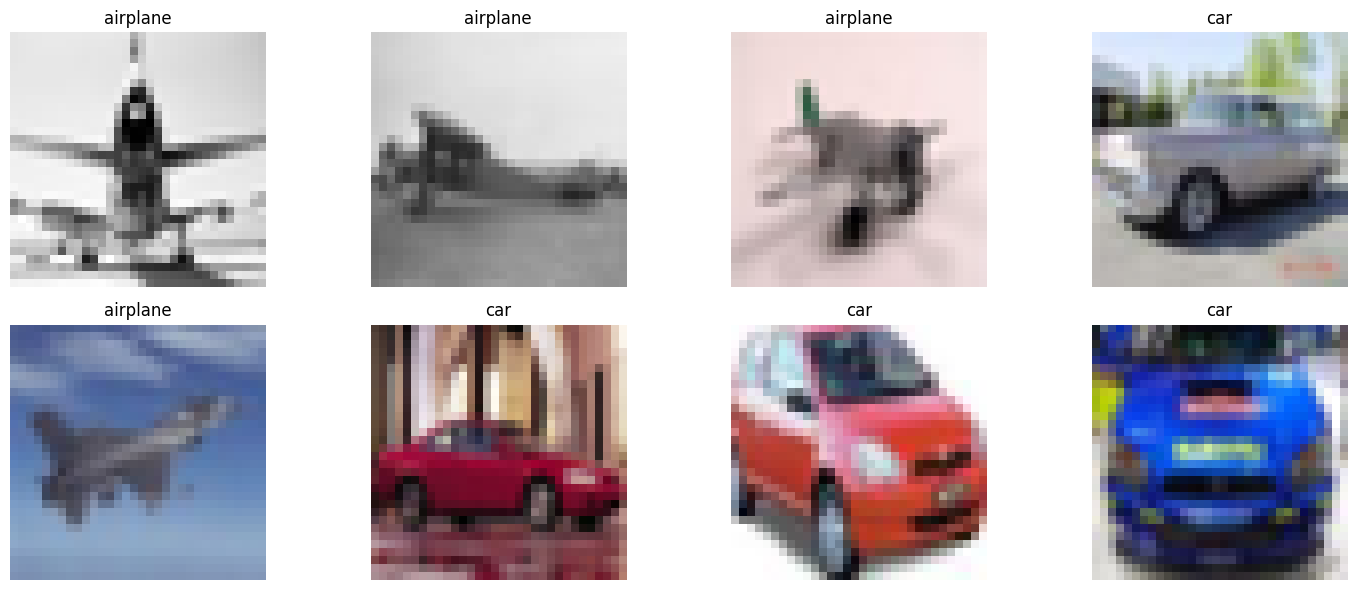
\includegraphics[width=0.9\textwidth]{imgs/introduction/amostra.png}
    \caption{Amostra do banco de imagens}
    \label{fig:amostra} % cria um rótulo para referência no texto
\end{figure}


O banco de imagens utilizado foi importado da classe \texttt{datasets.cifar10} da biblioteca \texttt{Keras} através da função \texttt{load\_data()}. A escolha de usar um mesmo banco de dados em todas as questões tem como intuito realizar uma comparação entre as diferentes estratégias de classificação dos dados que cada exercício pede.

%=================================================================================================
%=================================================================================================
%=================================================================================================
%=================================================================================================
%=================================================================================================
%=================================================================================================
%=================================================================================================
%=================================================================================================
%=================================================================================================
%=================================================================================================
%=================================================================================================


\section*{\textbf{Pré-processamento}}
\addcontentsline{toc}{section}{Pré-processamento}

Para a realização dos exercícios 1 e 3, foi realizado um pré-processamento dos dados, necessário para a execução das operações necessárias nestas questões.

As seguintes operações foram realizadas:

\begin{itemize}
    \item Conversão para escala de cinza: realizada através da biblioteca \texttt{OpenCV}, utilizando a função \texttt{cvtColor};
    \item Vetorização das imagens: realizada através do método \texttt{reshape} da biblioteca \texttt{Numpy};
    \item Normalização das features: realizada através da ferramenta \texttt{StandardScaler} da biblioteca \texttt{Scikit-Learn}. O \texttt{StandardScaler} ajusta cada feature do conjunto de dados de acordo com a fórmula:
    
    \[
    z = \frac{x - \mu}{\sigma}
    \]
    
    Onde:
    \begin{itemize}
        \item \( x \) é o valor original da feature.
        \item \( \mu \) é a média dos valores da feature.
        \item \( \sigma \) é o desvio padrão da feature.
    \end{itemize}
    
\end{itemize}

Após isso, através da ferramenta \texttt{train\_test\_split} da biblioteca \texttt{Scikit-Learn}, o conjunto de dados foi separado com proporção de 70\% para treinamento e 30\% para teste. Além disso, com o intuito de realizar a comparação sob o mesmo conjunto de dados para todas as questões, foi selecionada a opção \texttt{random\_state} = 42 na função utilizada para a separação dos dados, fixando a semente de sorteio dos dados. Na implementação de cada uma das questões foi realizado o cálculo da quantidade de imagens de cada classe no conjunto de treinamento, com o intuito de observar possíveis desbalanceamentos de dados. Como mostra a Figura \ref{fig:distri}, as duas classes tinham números de dados iguais, não sendo necessário, portanto, a exclusão ou adição de novos dados no conjunto de treinamento para a realização dos exercícios.

\begin{figure}[H]
    \centering 
    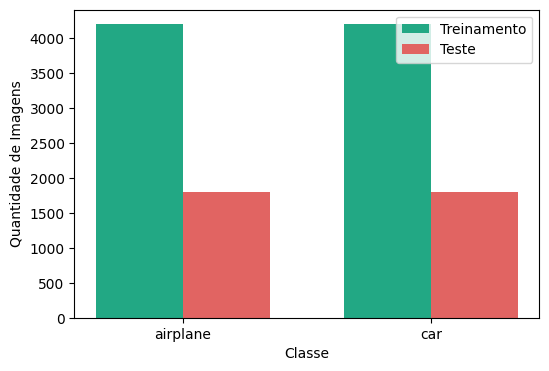
\includegraphics[width=0.4\textwidth]{imgs/introduction/distri.png}
    \caption{Histograma da quantidade de imagens por classe para treinamento e teste}
    \label{fig:distri} % cria um rótulo para referência no texto
\end{figure}


%=================================================================================================
%=================================================================================================
%=================================================================================================
%=================================================================================================
%=================================================================================================
%=================================================================================================
%=================================================================================================
%=================================================================================================
%=================================================================================================
%=================================================================================================
%=================================================================================================


\section*{\textbf{Questão 1}}
\addcontentsline{toc}{section}{Questão 1}

\textit{Considere um banco de dados de imagens e um problema de classificação. Aplique validação cruzada leave-one-out multi-fold explicada na seção 8.5 de \cite{book}, com $K = 4$, e SVM como segue:
    \begin{itemize}
        \item[(a)]SVM Linear não separável com espaço de características obtido através do KPCA.
        \item[(b)] SVM Kernel não separável com espaço de características obtido através do PCA.
        \item[(c)] Compare os resultados dos itens (a) e (b).
    \end{itemize}
}

Para a realização deste exercício, especificamente para o proposto na letra (a), foi inicialmente realizado o cálculo do Kernel Principal Component Analysis (KPCA) através da biblioteca \texttt{Scikit-Learn} com a função \texttt{KernelPCA}. O objetivo deste passo é determinar o número de componentes principais de todas as bases que serão calculadas posteriormente para cada fold. Logo, foi empiricamente escolhido um kernel polinomial para o cálculo da matriz KPCA com todas as componentes, para posteriormente determinar o número de componentes principais. Apenas como ilustração, o conjunto de dados de treinamento projetados nas duas principais componentes do KPCA está presente na Figura \ref{fig:KPCA}.

\begin{figure}[H]
    \centering 
    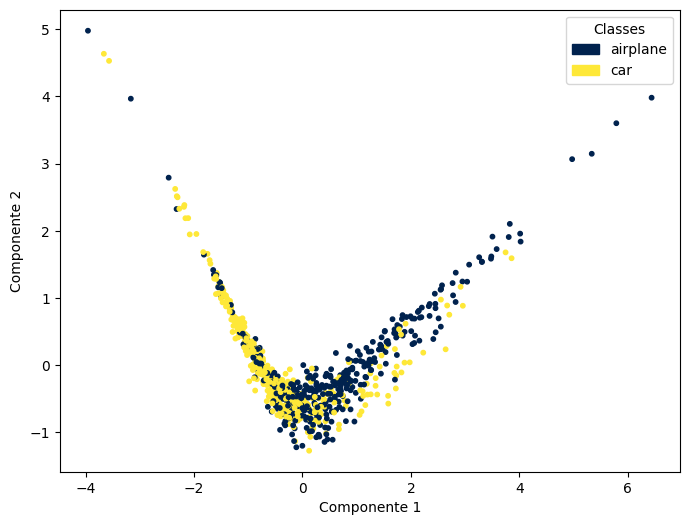
\includegraphics[width=0.4\textwidth]{imgs/ex1/KPCA.png}
    \caption{Projeção do conjunto de treinamento na base obtida pelo KPCA}
    \label{fig:KPCA} % cria um rótulo para referência no texto
\end{figure}

A função para calcular a base KPCA também retorna os autovalores correspondentes aos autovetores que formam as colunas da base KPCA obtida no espaço de características. Assim, foi possível calcular a variância explicada dividindo cada autovalor pela soma de todos os autovalores, que estão em ordem decrescente. Utilizando a biblioteca \texttt{Matplotlib}, foi gerado o gráfico mostrado na Figura \ref{fig:vari_kpca}, que ilustra a soma cumulativa das variâncias explicadas. Esse gráfico permite avaliar o número de componentes da base KPCA necessários para representar uma certa porcentagem da variância total do conjunto de dados.

Para determinar a quantidade ideal de componentes principais, utilizou-se a biblioteca \texttt{Numpy} com a função \texttt{argmax} para calcular o número de componentes necessários para explicar no mínimo 95\% da variância dos dados, com base na variância explicada cumulativa. O resultado indicou que, neste caso, são necessários 435 componentes.

\begin{figure}[H]
    \centering 
    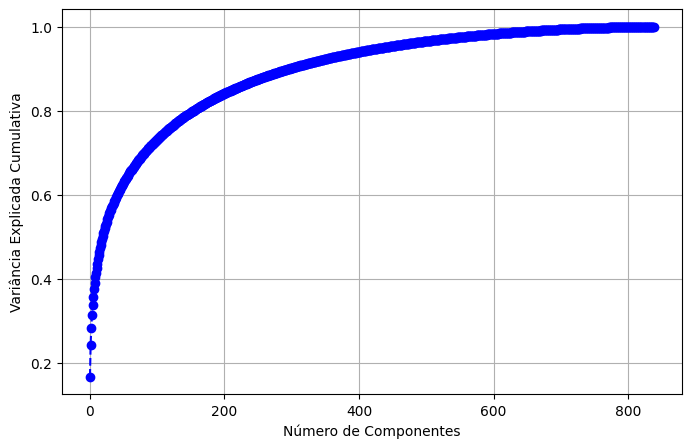
\includegraphics[width=0.5\textwidth]{imgs/ex1/vari_kpca.png}
    \caption{Gráfico da variância explicada cumulativa por componentes KPCA}
    \label{fig:vari_kpca} % cria um rótulo para referência no texto
\end{figure}

Utilizando a técnica de K-Fold Cross-Validation, os dados são divididos em \( k \) subconjuntos (ou "folds") de tamanhos aproximadamente iguais. Em cada iteração, um dos \( k \) folds é reservado como conjunto de validação, enquanto os \( k-1 \) folds restantes são utilizados para treinamento, resultando em \( k \) modelos distintos. Para a resolução deste exercício, foi utilizado \( \texttt{K-fold} = 4 \), sendo então realizado o cálculo da base KPCA para o conjunto de treinamento correspondente a cada fold, através da função \texttt{.fit()}, reduzindo a dimensionalidade deste conjunto de acordo com o número de componentes encontradas anteriormente, neste caso, 435. Posteriormente, foi realizada a projeção dos dados de treinamento, validação e testes nesta base através da função \texttt{pca.tranform()}. Logo após, a função \texttt{SVC} da biblioteca \texttt{Scikit-Learn} foi empregada para calcular o modelo de Máquinas de Vetores de Suporte (SVM), para o caso não separável, com o objetivo de realizar a classificação dos dados. Esta construção é baseada na minimização da função custo $\tau$ decrita abaixo:
\[
\tau(\phi, \xi, C) = \frac{1}{2} \|\phi\|^2 + C \sum_{i=1}^{M} \xi_i
\]
Onde:
\begin{itemize}
    \item \(\frac{1}{2} \|\phi\|^2\): É o termo de regularização que controla a complexidade do modelo, minimizando o valor dos pesos (norma de \(\phi\)).
    \item \(C\): É um hiperparâmetro que controla o trade-off entre a margem da fronteira de decisão e os erros de classificação. Valores maiores de \(C\) dão mais ênfase à minimização dos erros \(\xi_i\), enquanto valores menores favorecem uma maior margem com a penalização menor dos erros.
    \item \(\sum_{i=1}^{M} \xi_i\): Soma das variáveis de erro (\(\xi_i\)), que representam a quantidade pela qual as amostras violam a margem suave. Quanto maior a soma dessas variáveis, maior é o número de amostras classificadas incorretamente ou dentro da margem.
    \item \(M\): O número total de amostras.
\end{itemize}

Foi utilizado a constante $C=1$ para a realização desta questão, definida experimentalmente.

Os resultados obtidos refentes à acurácia da classificação dos modelos de cada fold, aplicados, tanto no conjunto de validação quanto no conjunto de teste, estão apresentados na Tabela \ref{tab:kpca_svm}. Em média, observa-se que o classificador apresentou uma maior acurácia nos conjuntos de teste em comparação com os conjuntos de validação, obtendo, em ambos casos, acurácias superiores à casa dos 78\%, chegando a 84\% no conjunto de testes.

\begin{table}[H]
    \centering
    \begin{tabular}{|c|c|c|c|c|c|}
    \hline
    \rowcolor[HTML]{C0C0C0} 
    Conjunto                          & Fold 1 & Fold 2 & Fold 3 & Fold 4 & Média  \\ \hline
    \cellcolor[HTML]{C0C0C0}Validação & 0.79   & 0.78   & 0.79   & 0.80   & 0.79  \\ \hline
    \cellcolor[HTML]{C0C0C0}Teste     & 0.83   & 0.84   & 0.81   & 0.84   & 0.83 \\ \hline
    \end{tabular}
    \caption{Acurácia da classificação do SVM Linear com o KPCA}
    \label{tab:kpca_svm}
\end{table}

Com o intuito de promover uma visualização gráfica para exemplificar como seria a reta de separação para apenas as duas principais componentes obtidas pelo cálculo do KPCA, foi realizado o treinamento de um novo SVM linear sobre o conjunto de dados projetados apenas nas duas principais componentes do KPCA, obtendo a reta de separação mostrada na Figura \ref{fig:kpca_reta}, juntamente com a projeção do conjunto de teste nesta base. Neste caso, a acurácia média obtida no conjunto de testes foi de 69\%, inferior à de 79\% obtida em média anteriormente com todas as componentes principais, evidenciando que a redução de dimensionalidade para apenas duas componentes principais impactou negativamente na performance do classificador. Além disso, a margem de separação construída possui um tamanho considerável, que indica que, nesta região, o classificador teve muita incerteza ao apontar de qual classe eram os dados.

\begin{figure}[H]
    \centering 
    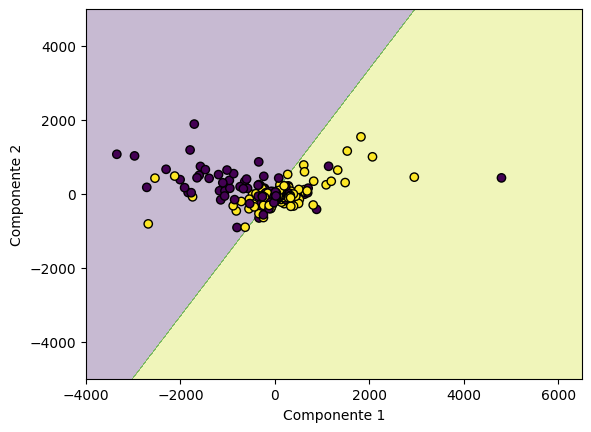
\includegraphics[width=0.5\textwidth]{imgs/ex1/kpca_reta.png}
    \caption{Reta de decisão do SVM Linear com KPCA}
    \label{fig:kpca_reta} % cria um rótulo para referência no texto
\end{figure}

\newpage

Para a realização do item (b), foi inicialmente realizado o cálculo do Principal Component Analysis (PCA) utilizando a biblioteca \texttt{Scikit-Learn} com a função \texttt{PCA}, também com o intuito de determinar o número de componentes principais para todas as bases PCA que serão calculadas em cada fold. Neste primeiro passo, foram calculadas todas as componentes principais, permitindo posteriormente a seleção das mais relevantes para este conjunto de dados. A projeção do conjunto de dados na base PCA está representada na Figura \ref{fig:PCA}.

\begin{figure}[H]
    \centering 
    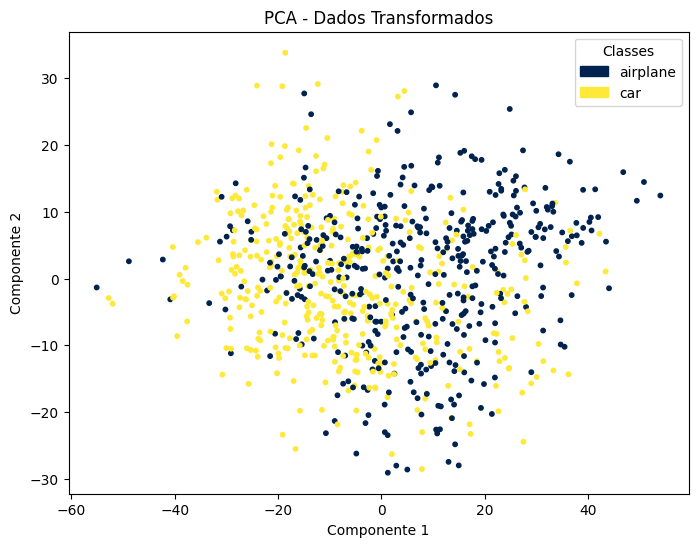
\includegraphics[width=0.5\textwidth]{imgs/ex1/PCA.png}
    \caption{Projeção do conjunto de treinamento na base PCA}
    \label{fig:PCA} % cria um rótulo para referência no texto
\end{figure}

Após o cálculo das componentes principais, foi gerado o gráfico da variância explicada cumulativa, fornecido pelo próprio cálculo do PCA através do método \texttt{explained\_variance\_ratio\_}. O resultado obtido está ilustrado na Figura \ref{fig:vari_pca}. Para selecionar o número adequado de componentes principais, foi utilizada a função \texttt{argmax} da biblioteca \texttt{Numpy}, determinando o número de componentes necessárias para explicar pelo menos 95\% da variância dos dados, resultando em 123 componentes. Com isso, a matriz de dados transformada pelo PCA de cada fold será reduzida para este número de componentes principais.

\begin{figure}[H]
    \centering 
    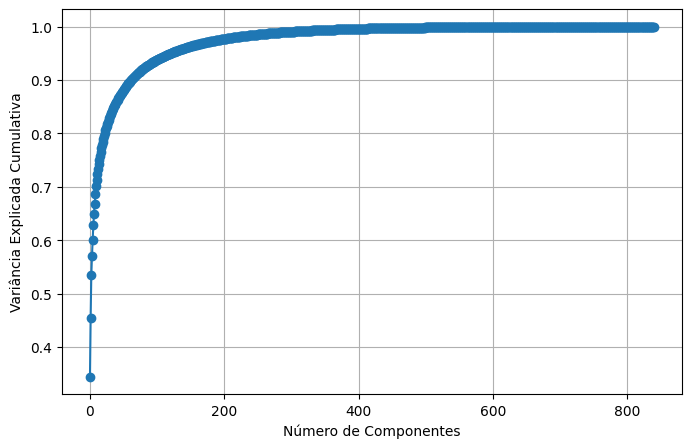
\includegraphics[width=0.5\textwidth]{imgs/ex1/vari_pca.png}
    \caption{Gráfico da variância explicada cumulativa para as componentes do PCA}
    \label{fig:vari_pca} % cria um rótulo para referência no texto
\end{figure}

Em seguida, foi aplicada a estratégia \texttt{K-fold} com valor 4, com a mesma subdivisão de dados realizada no item (a), para que fosse posteriormente realizada uma comparação entre os modelos. Novamente, foi realizado o cálculo de PCA para o conjunto de treinamento respectivo ao fold através da função \texttt{.fit()}, e então reduzindo a dimensionalidade para as 123 componentes principais. Utilizando a função \texttt{SVC} da biblioteca \texttt{Scikit-Learn}, foi construído um Kernel Support Vector Machine (KSVM), com kernel polinomial definido empiricamente, com o objetivo de realizar a classificação dos dados, obtendo as acurácias mostradas na Tabela \ref{tab:pca_svm} para os conjuntos de validação e teste. Novamente, a constante de regularização considerada foi \(C=1\), definida experimentalmente.

\begin{table}[H]
    \centering
    \begin{tabular}{|c|c|c|c|c|c|}
    \hline
    \rowcolor[HTML]{C0C0C0} 
    Conjunto                          & Fold 1 & Fold 2 & Fold 3 & Fold 4 & Média  \\ \hline
    \cellcolor[HTML]{C0C0C0}Validação & 0.82   & 0.69   & 0.73   & 0.74   & 0.745  \\ \hline
    \cellcolor[HTML]{C0C0C0}Teste     & 0.83   & 0.83   & 0.77   & 0.81   & 0.81 \\ \hline
    \end{tabular}
    \caption{Acurácia da classificação do KSVM Polinomial com o PCA}
    \label{tab:pca_svm}
\end{table}

Com o intuito de visualizar o plano de separação utilizando apenas as duas componentes principais obtidas pelo PCA, foi treinado um novo SVM com kernel polinomial sobre o conjunto de treinamento projetado na base PCA reduzida apenas para suas duas componentes principais, gerando a curva de separação presente na Figura \ref{fig:pca_reta}. Essa figura também mostra a projeção do conjunto de testes nas duas primeiras direções principais. Nesse cenário, a acurácia média alcançada no conjunto de teste foi de 64\%, evidenciando mais uma vez que a redução de dimensionalidade para duas componentes impactou negativamente na acurácia do classificador.

\begin{figure}[H]
    \centering 
    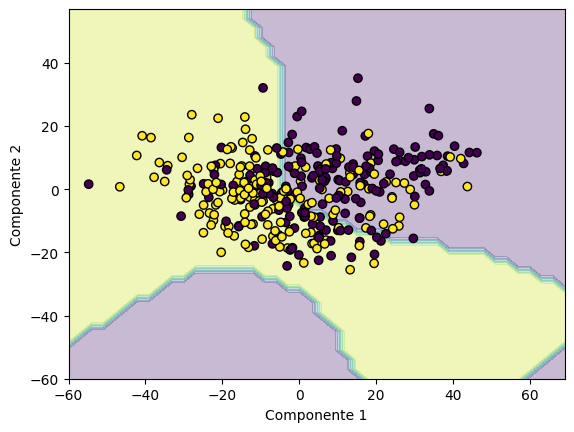
\includegraphics[width=0.5\textwidth]{imgs/ex1/pca_reta.png}
    \caption{Curva de decisão do KSVM Polinomial com PCA}
    \label{fig:pca_reta} % cria um rótulo para referência no texto
\end{figure}

Observando as Tabelas \ref{tab:kpca_svm} e \ref{tab:pca_svm}, podemos notar que, no geral, o modelo proposto no item (a) obteve uma maior acurácia na classificação das imagens, tanto no conjunto de treinamento quanto no de conjunto de validação. Além disso, a matriz de confusão presente na Figura \ref{fig:1conf_b}, construída sobre o conjunto de testes, mostra que, por exemplo, para o fold igual a 3 no modelo proposto no item (b), houve uma quantidade significativa de predições erradas, onde aviões foram preditos como carros. Este problema não ocorreu de maneira intensa no modelo proposto no item (a), como mostrado na Figura \ref{fig:1conf_a}, o que também evidencia sua performence superior na tarefa em questão.

\begin{figure}[H]
    \centering 
    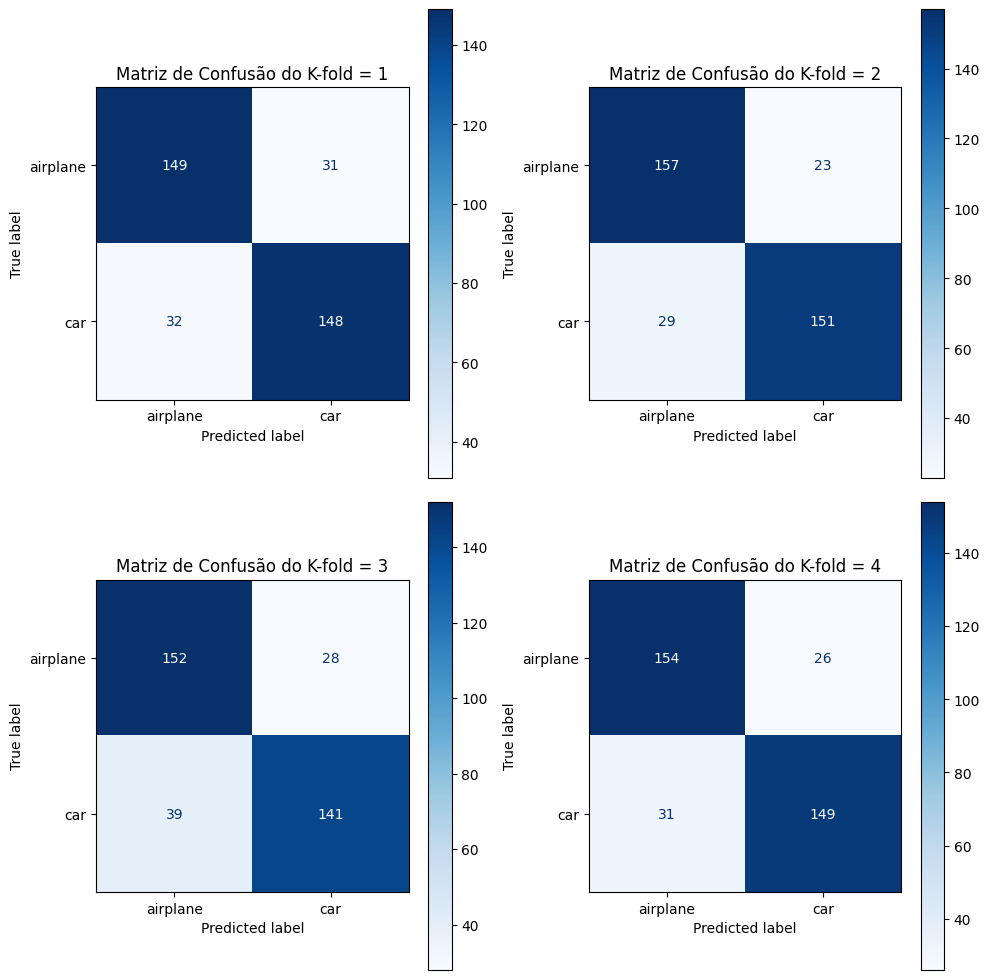
\includegraphics[width=0.62\textwidth]{imgs/ex1/conf_a.png}
    \caption{Matriz de confusão dos modelos do item (a) aplicados ao conjunto de testes}
    \label{fig:1conf_a} % cria um rótulo para referência no texto
\end{figure}

\begin{figure}[H]
    \centering 
    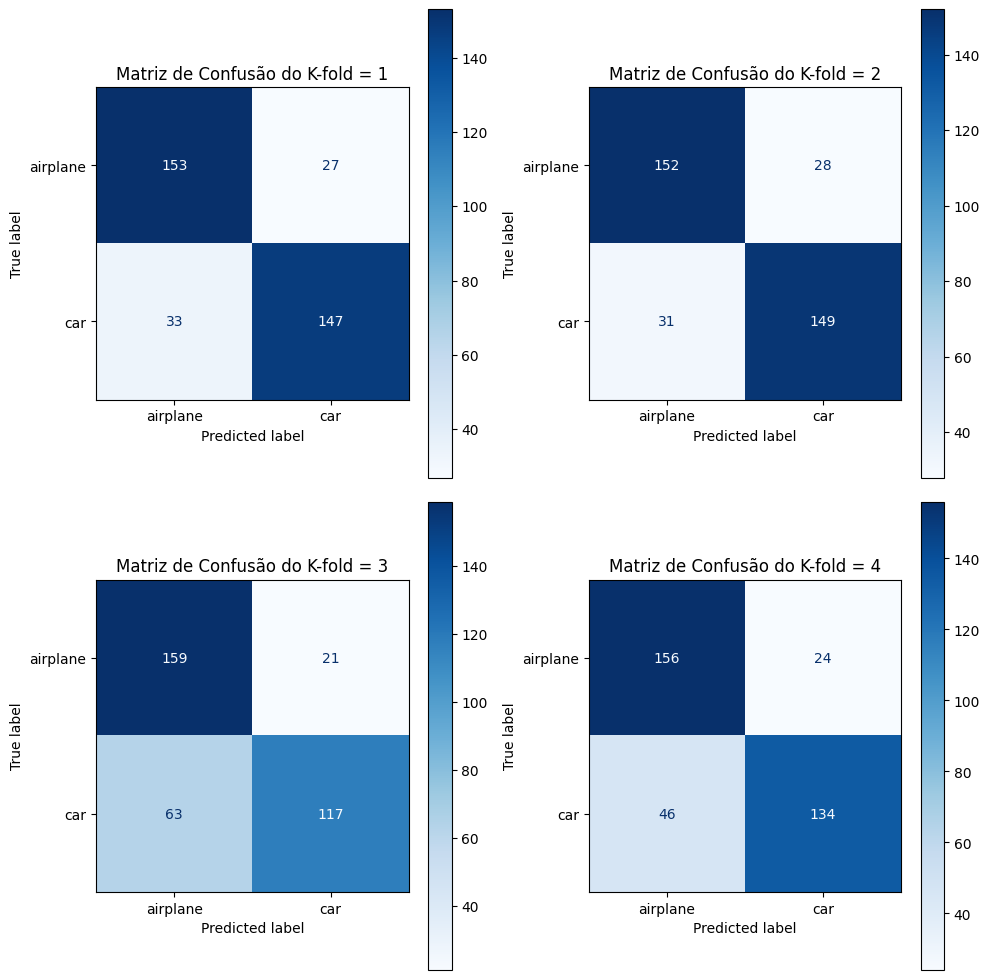
\includegraphics[width=0.62\textwidth]{imgs/ex1/conf_b.png}
    \caption{Matriz de confusão dos modelos do item (b) aplicados ao conjunto de testes}
    \label{fig:1conf_b} % cria um rótulo para referência no texto
\end{figure}

Para acessar o código referente à realização deste exercício, \href{https://github.com/lorran-araujo/LNCC/blob/main/disciplinas/redes-neurais/codes/lista3/exercicio1.ipynb}{clique aqui}.

%=================================================================================================
%=================================================================================================
%=================================================================================================
%=================================================================================================
%=================================================================================================
%=================================================================================================
%=================================================================================================
%=================================================================================================
%=================================================================================================
%=================================================================================================
%=================================================================================================



\section*{\textbf{Questão 2}}
\addcontentsline{toc}{section}{Questão 2}

\textit{Considere um banco de dados e um problema de classificação. Aplique a validação cruzada multi-fold leave-one-out explicada na seção 8.5 de \cite{book}, com $K = 5$, para um modelo de CNN. Utilize as facilidades disponíveis em bibliotecas para a implementação de redes neurais, como Keras, TensorFlow, etc.}

\textit{\begin{enumerate}
    \item[(a)] Mostre a representação gráfica da evolução das etapas de treinamento e validação (ver Figura 8.8 da monografia do curso).
    \item[(b)] Realize uma análise estatística do desempenho (seção 8.6) dos cinco modelos aplicados sobre a $\mathbb{D}_{te}$.
\end{enumerate}}


Para a realização deste exercício, foram utilizadas todas as 12.000 imagens da base de dados CIFAR-10 referentes às classes aviões e carros. 

O modelo da Rede Neural Convolucional (CNN) foi construído empiricamente, com arquitetura inspirada na rede Virtual Geometry Group Network (VGGNet), criada por Simonyan e Zisserman, pesquisadores da Universidade de Oxford, em 2014. A principal inovação da VGGNet foi o uso de blocos de convolução com filtros de tamanho 3x3, onde essa arquitetura ajudou a melhorar a precisão das classificações \cite{simonyan2014very}. 

A arquitetura construída com essa inspiração está descrita na Tabela \ref{tab:arquiCNN}.

\begin{table}[H]
    \centering
    \begin{tabular}{|c|c|c|c|c|c|}
    \hline
    \rowcolor[HTML]{C0C0C0} 
    Camadas                                                  & Tipo          & Filtros/Neurônios & Tam. do filtro & Padding & F. Ativação \\ \hline
    \cellcolor[HTML]{C0C0C0}                                 & Convolucional & 32                   & (3,3)             & same    & ReLU        \\ \cline{2-6} 
    \cellcolor[HTML]{C0C0C0}                                 & Convolucional & 32                   & (3,3)             & same    & ReLU        \\ \cline{2-6} 
    \multirow{-3}{*}{\cellcolor[HTML]{C0C0C0}1ª Conv e Pool} & Max Pooling   & -                    & (2,2)             & -       & -           \\ \hline
    \cellcolor[HTML]{C0C0C0}                                 & Convolucional & 64                   & (3,3)             & same    & ReLu        \\ \cline{2-6} 
    \cellcolor[HTML]{C0C0C0}                                 & Convolucional & 64                   & (3,3)             & same    & ReLU        \\ \cline{2-6} 
    \multirow{-3}{*}{\cellcolor[HTML]{C0C0C0}2ª Conv e Pool} & Max Pooling   & -                    & (2,2)             & -       & -           \\ \hline
    \cellcolor[HTML]{C0C0C0}                                 & Convolucional & 128                  & (3,3)             & same    & ReLU        \\ \cline{2-6} 
    \cellcolor[HTML]{C0C0C0}                                 & Convolucional & 128                  & (3,3)             & same    & ReLU        \\ \cline{2-6} 
    \multirow{-3}{*}{\cellcolor[HTML]{C0C0C0}3ª Conv e Pool} & Max Pooling   & -                    & (2,2)             & -       & -           \\ \hline
    \cellcolor[HTML]{C0C0C0}Flatten                          & Flatten       & -                    & -                 & -       & -           \\ \hline
    \cellcolor[HTML]{C0C0C0}Dense                            & Dense         & 512                  & -                 & -       & ReLU        \\ \hline
    \cellcolor[HTML]{C0C0C0}Saída                            & Dense         & 2                    & -                 & -       & Softmax     \\ \hline
    \end{tabular}
    \caption{Arquitetura do modelo da rede CNN}
    \label{tab:arquiCNN}

\end{table}

Logo, foram usadas no total 6 camadas do tipo convolucionais, 3 camadas de pooling e uma camada densa Multi Layer Perceptron (MLP), onde:

\begin{itemize}
    \item A função de ativação Rectified Linear Unit(ReLU) foi utilizada na camada Dense e na saída das camadas convolucionais, após o batch normalization, como na arquitetura da VGGNet. A função é dada por:
    
    \[
    \text{ReLu}(x) = \max(0, x).
    \]

    \item A função Softmax foi usada na última camada. Geralmente ela é utilizada para problemas de
    classificação multiclasse. Ela transforma os valores de entrada em uma distribuição de probabili-
    dade, onde cada valor de saída é interpretado como a probabilidade da entrada pertencer a uma
    das classes. A função Softmax é definida como:
    \[
        \text{softmax}(\mathbf{z}) = \left( \frac{\exp(z_1)}{\sum_{j=1}^{K} \exp(z_j)}, \frac{\exp(z_2)}{\sum_{j=1}^{K} \exp(z_j)}, \ldots, \frac{\exp(z_K)}{\sum_{j=1}^{K} \exp(z_j)} \right).
    \]
    
    \item Foi utilizado o parâmetro das redes convolucionais padding igual a same, que significa que haverá um preenchimento uniforme nas bordas com zeros, e strides igual a 1, de modo que as saídas das camadas convolucionais terão o mesmo tamanho que suas entradas \cite{keras}.
\end{itemize}

Foram usadas também algumas outras estratégias para obter uma melhor perfomance da rede, como:

\begin{itemize}
    \item Batch Normalization: técnica usada para melhorar a estabilidade e a velocidade do treinamento de redes neurais profundas. Ela funciona normalizando a entrada de cada camada para ter média zero e variância unitária. A ideia é normalizar as saídas das camadas para que estejam em uma faixa específica, o que permite que o treinamento seja mais estável e rápido \cite{ioffe2015batch}. Camadas de batch normalization foram aplicadas nas saídas de todas as camadas CNN e Dense.
    \item Dropout: técnica de regularização usada para prevenir o overfitting em redes neurais. Durante o treinamento, o dropout desativa aleatoriamente uma fração dos neurônios em uma camada, forçando a rede a aprender representações mais robustas e a não depender excessivamente de nenhum neurônio específico. Isso faz com que a rede neural generalize melhor, pois cada unidade não pode confiar excessivamente em outras unidades \cite{srivastava2014dropout}. Para este modelo, um dropout de 25\% foi aplicado a última camada da primeira, segunda e terceira camada Conv e Pool. Além disso, foi usado um dropout de 50\% na camada Dense.
\end{itemize}

Para função de perda (Loss), foi utilizada a categorical cross-entropy (CCE), que é usada para problemas de classificação multiclasse. Ela mede a divergência entre a distribuição de probabilidade prevista pela rede (saída do softmax) e a verdadeira distribuição de rótulos. A CCE é definida da seguinte forma:

\[
\text{CCE} = -\dfrac{1}{N}\sum_{i=1}^{N} \sum_{j=1}^{C} y_{ij} \log(\hat{y}_{ij})
\]

onde:

\begin{itemize}
    \item \(N\): é o número de amostras no conjunto de dados.
    \item \(C\): é o número de classes.
    \item \(y_{ij}\): é o rótulo verdadeiro para a \(i\)-ésima amostra e a \(j\)-ésima classe. Em uma codificação one-hot, \(y_{ij}\) é 1 se a amostra \(i\) pertence à classe \(j\), e 0 caso contrário.
    \item \(\hat{y}_{ij}\): é a probabilidade prevista pelo modelo de que a \(i\)-ésima amostra pertence à \(j\)-ésima classe. Este valor é a saída do modelo após a aplicação da função softmax. 
\end{itemize}

O otimizador utilizado foi o Stocastic Gradiente Descendent (SGD), considerando learning rate igual a 0.001 e um momentum igual a 0.9. Logo, a atualização dos pesos será dada da seguinte forma \cite{keras}:

\[
velocity = velocity - learning\_rate * g 
\]

\[
w = w + velocity
\]

onde \(g\) é o gradiente da função Loss. Além disso, foi utilizada a regularização \( L^2 \) com parâmetro \(\lambda = 1e-6\), a qual adiciona um termo de penalização à função de perda original, que ajuda a manter os pesos da rede menores e mais controlados, pois estes são considerados na função de perda. Logo, a função Loss com o termo de regularização é dada por:

\[
\text{Loss} = CCE + \dfrac{\lambda}{2} \sum_{i=1}^{n} w_i^2
\]

onde \(\lambda\) é o parâmetro de regularização e \(w_i\) são os pesos do modelo. 

A inicialização dos pesos é realizada através de uma distribuição uniforme, denominada Glorot Uniform. O intervalo do qual os pesos são amostrados é definido por:

\[
w \sim \mathcal{U}\left(-\sqrt{\frac{6}{n_{\text{in}} + n_{\text{out}}}}, \sqrt{\frac{6}{n_{\text{in}} + n_{\text{out}}}}\right)
\]

Onde:
\begin{itemize}
    \item \( w \) são os pesos.
    \item \( n_{\text{in}} \) é o número de unidades de entrada da camada (ou seja, o número de neurônios na camada anterior).
    \item \( n_{\text{out}} \) é o número de unidades de saída da camada (ou seja, o número de neurônios na camada atual).
    \item \( \mathcal{U}(a, b) \) representa uma distribuição uniforme entre \( a \) e \( b \).
\end{itemize}

Já os bias são inicializados com valores iguais a zero.

Para o treinamento do modelo, utilizando a biblioteca \texttt{Keras}, foi considerada uma estratégia de early stopping da classe \texttt{callbacks} da função \texttt{fit} para evitar overfitting. Considerando a métrica de loss da validação como a quantidade a ser monitorada no early stopping, temos que os seguinte parâmetros para este critério de parada foram utilizados:

\begin{itemize}
    \item \textit{min\_delta} = 0.0001:  quantidade mínima para ser considerada como melhoria;
    \item \textit{patience} = 6: número de épocas sem melhorias a quais o treinamento será interrompido;
    \item \textit{restore\_best\_weights} = True: restaura para a rede os pesos referentes à epoca com melhor resultado na métrica escolhida.
\end{itemize}

Finalmente, foi realizado o treinamento do modelo usando $K-Fold$ = 5, como determinado pela questão. Para isso, foi considerado o batch size tamanho 64 e 50 épocas, definidos empiricamente. A evolução da acurácia e da loss, para o treinamento e a validação, estão presentes nos gráficos das figuras \ref{fig:t1}, \ref{fig:t2}, \ref{fig:t3},\ref{fig:t4} e \ref{fig:t5} . Através do gráfico, podemos perceber no geral que a evolução da loss não demonstrou a ocorrência de overfitting, mas pode se notar uma oscilação na acurácia do conjunto de validação do treinamento.

\begin{figure}[H]
    \centering 
    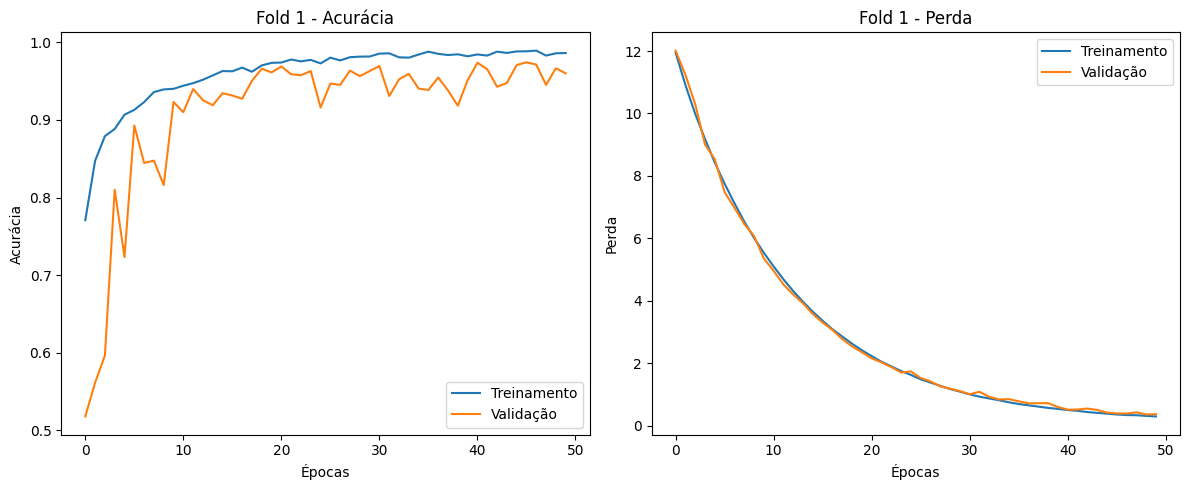
\includegraphics[width=0.75\textwidth]{imgs/ex2/train_f1.png}
    \caption{Evolução da acurácia e da loss do conjunto de treinamento e de validação para o fold 1}
    \label{fig:t1} % cria um rótulo para referência no texto
\end{figure}

\begin{figure}[H]
    \centering 
    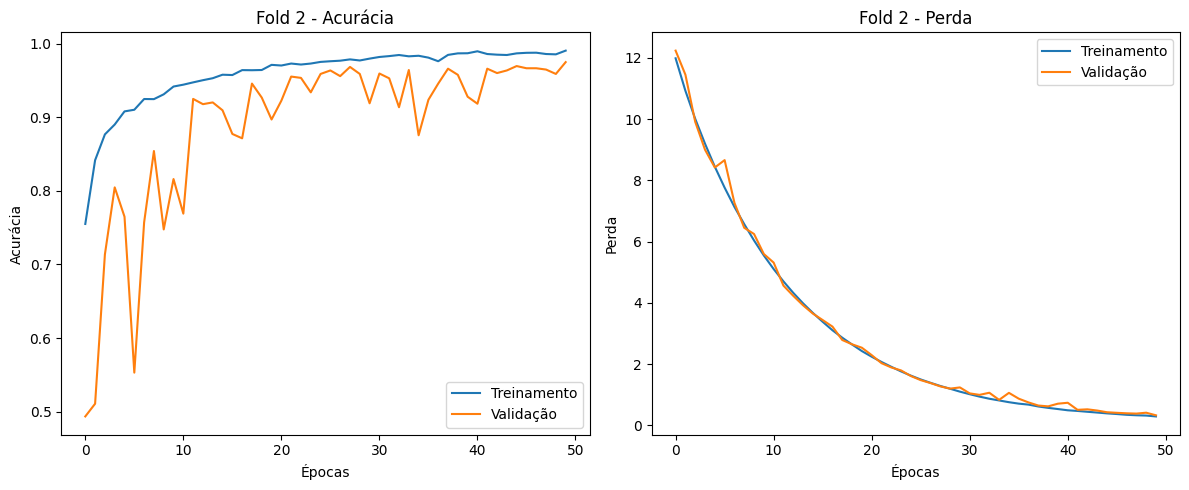
\includegraphics[width=0.75\textwidth]{imgs/ex2/train_f2.png}
    \caption{Evolução da acurácia e da loss do conjunto de treinamento e de validação para o fold 2}
    \label{fig:t2} % cria um rótulo para referência no texto
\end{figure}

\begin{figure}[H]
    \centering 
    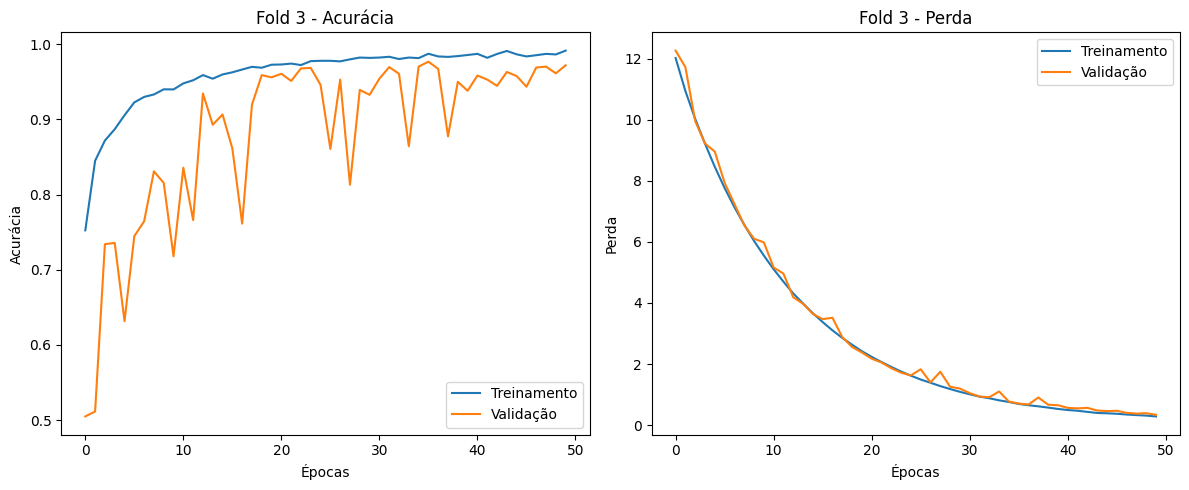
\includegraphics[width=0.75\textwidth]{imgs/ex2/train_f3.png}
    \caption{Evolução da acurácia e da loss do conjunto de treinamento e de validação para o fold 3}
    \label{fig:t3} % cria um rótulo para referência no texto
\end{figure}

\begin{figure}[H]
    \centering 
    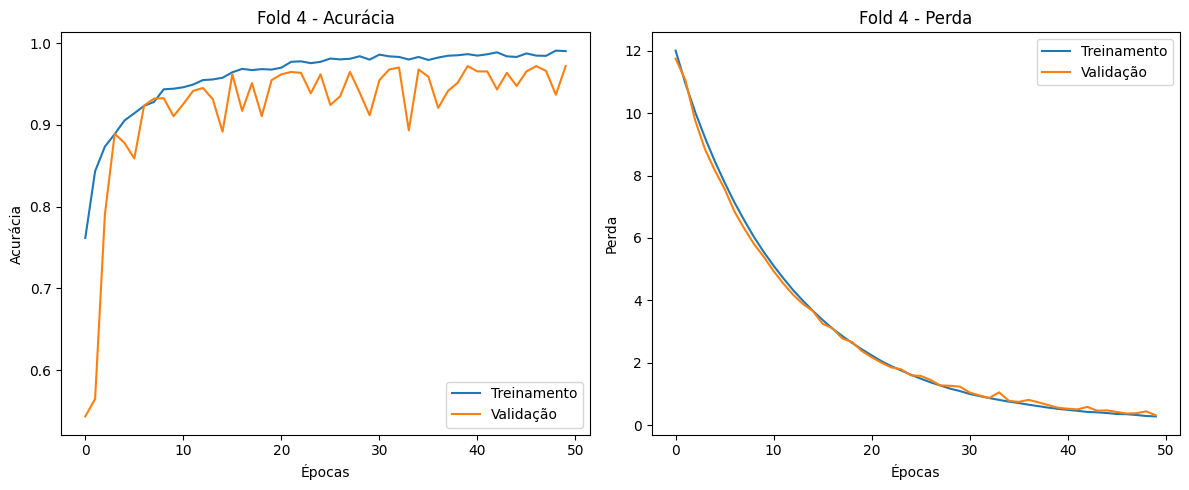
\includegraphics[width=0.75\textwidth]{imgs/ex2/train_f4.png}
    \caption{Evolução da acurácia e da loss do conjunto de treinamento e de validação para o fold 4}
    \label{fig:t4} % cria um rótulo para referência no texto
\end{figure}

\begin{figure}[H]
    \centering 
    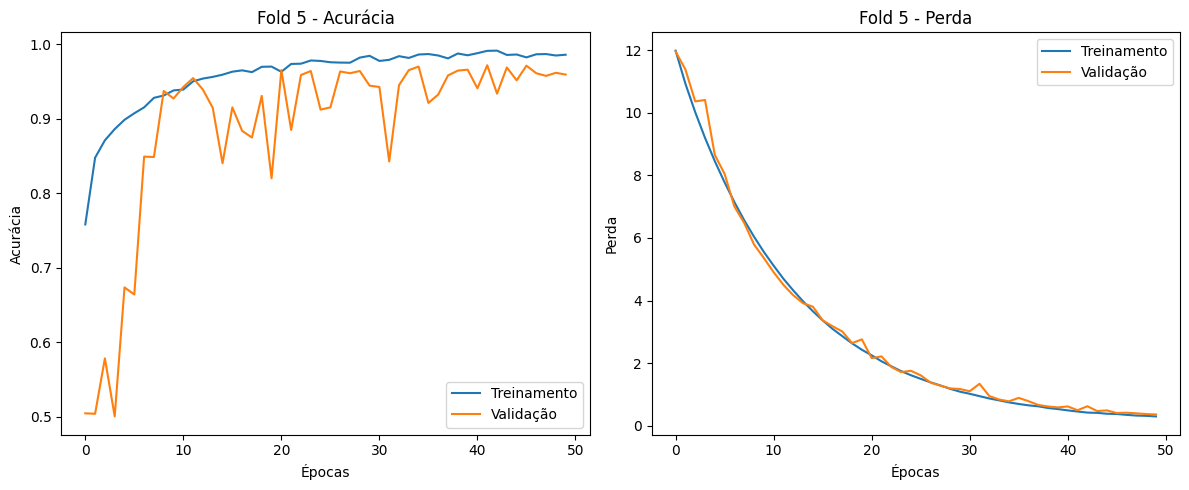
\includegraphics[width=0.75\textwidth]{imgs/ex2/train_f5.png}
    \caption{Evolução da acurácia e da loss do conjunto de treinamento e de validação para o fold 5}
    \label{fig:t5} % cria um rótulo para referência no texto
\end{figure}

Os modelos apresentaram uma acurácia final média de 97\% sobre o conjunto de validação. Com as ferramentas \texttt{confusion\_matrix} e \texttt{classification\_report}, presentes na biblioteca \texttt{Scikit-Learn}, podemos então plotar a matriz de confusão relativa aos modelos respectivos à cada fold, presente na Figura \ref{fig:conf}, onde a legenda 0 se refere a aviões e a legenda 1 a carros, e também calcular as métricas estátisticas descritas na seção 8.6 de \cite{book}, com precisão de duas casas decimais, obtendo então os resultados, sobre o conjunto de teste, presentes na tabela \ref{tab:acu1}.

\begin{table}[H]
    \centering
    \begin{tabular}{|c|c|c|c|c|c|c|}
    \hline
    \rowcolor[HTML]{C0C0C0} 
    Métricas                          & K=1  & K=2  & K=3  & K=4  & K = 5 & Média \\ \hline
    Macro Precision of the classifier & 0.96 & 0.97 & 0.97 & 0.97 & 0.98 & 0.97  \\ \hline
    Macro Recal of the Classifier     & 0.96 & 0.97 & 0.97 & 0.97 & 0.97 & 0.97  \\ \hline
    Macro F1 score                    & 0.96 & 0.97 & 0.97 & 0.97 & 0.97 & 0.97  \\ \hline
    Multi-Class Acuracy               & 0.96 & 0.97 & 0.97 & 0.97 & 0.97 & 0.97  \\ \hline
    Averaged Error Rate                & 0.04 & 0.03 & 0.03 & 0.03 & 0.03 & 0.03  \\ \hline
    \end{tabular}
    \caption{Métricas de performance dos modelos aplicados ao conjunto de testes}
    \label{tab:acu1}
\end{table}

\begin{figure}[H]
    \centering 
    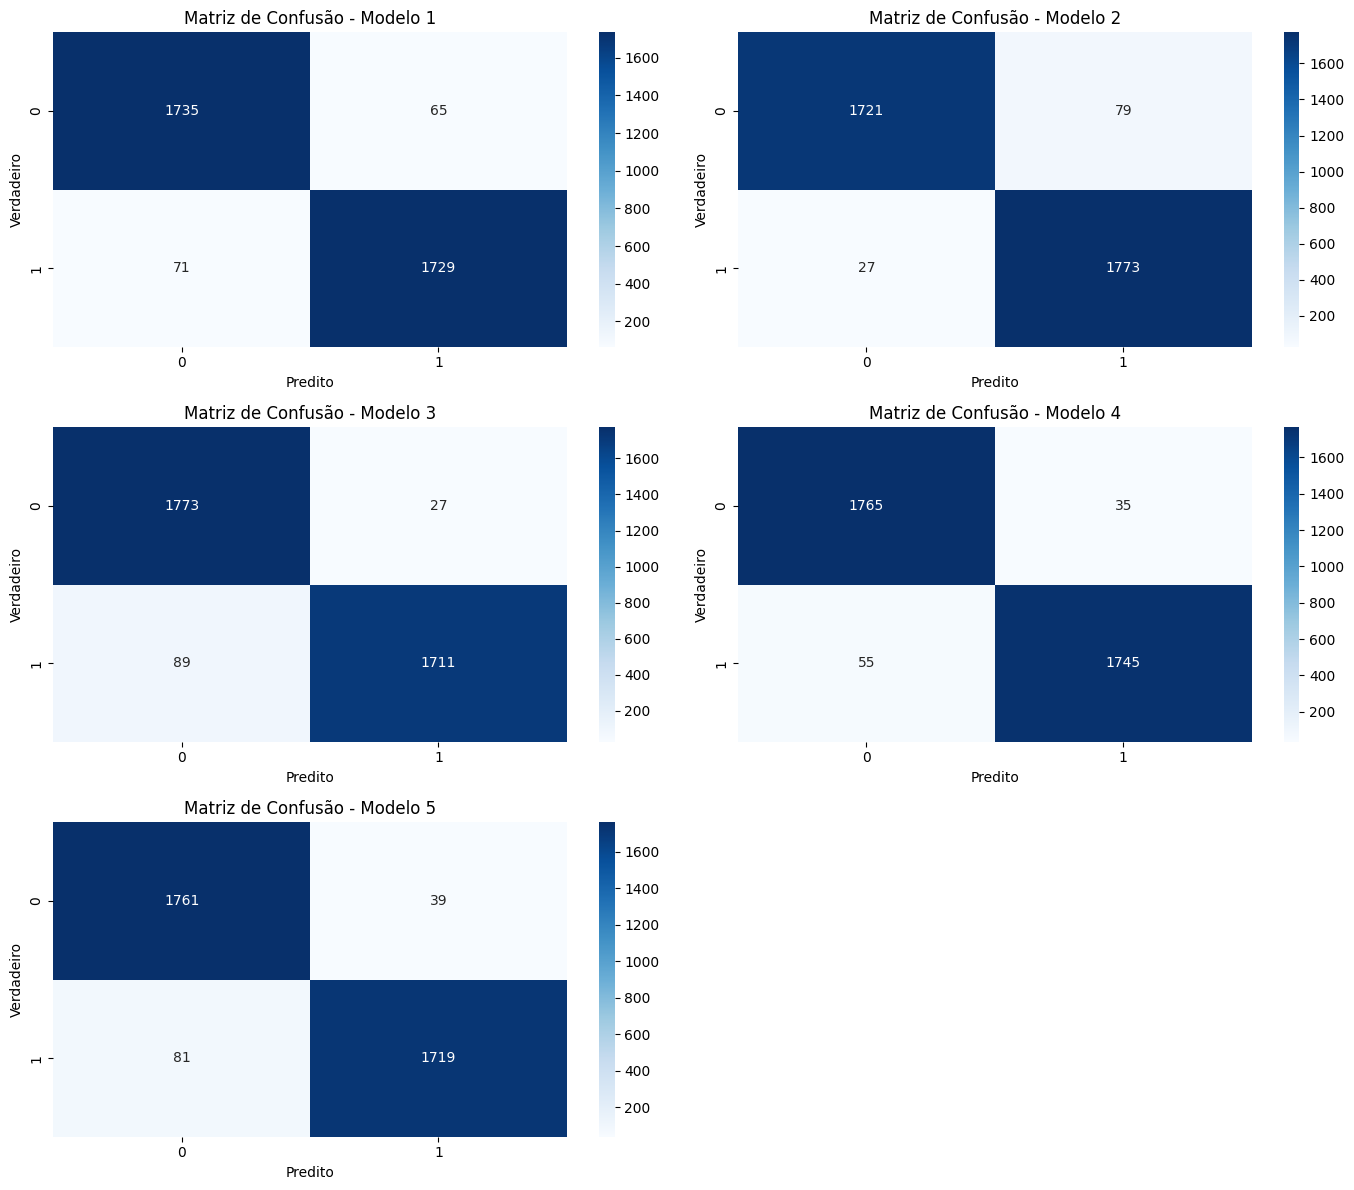
\includegraphics[width=0.95\textwidth]{imgs/ex2/confusion.png}
    \caption{Matriz de confusão dos modelos aplicados ao conjunto de testes}
    \label{fig:conf} % cria um rótulo para referência no texto
\end{figure}

Através dessas métricas, podemos observar que, no geral, os modelos se comportaram de maneira bastante semelhante, atingindo valores próximos para as métricas calculadas. A matriz de confusão também evidencia que não houve nenhuma classe com uma quantidade considerável de falsos positivos ou falsos negativos, resultando em uma ótima acurácia média de 97\%.

Para acessar o código referente à realização deste exercício, \href{https://github.com/lorran-araujo/LNCC/blob/main/disciplinas/redes-neurais/codes/lista3/exercicio2.ipynb}{clique aqui}.

%=================================================================================================
%=================================================================================================
%=================================================================================================
%=================================================================================================
%=================================================================================================
%=================================================================================================
%=================================================================================================
%=================================================================================================
%=================================================================================================
%=================================================================================================
%=================================================================================================

\section*{\textbf{Questão 3}}
\addcontentsline{toc}{section}{Questão 3}

\textit{Considere um banco de dados de imagens e um problema de classificação.}

\begin{enumerate}
    \item[(a)] \textit{ Aplique a validação cruzada multi-fold leave-one-out explicada na seção 8.5 de \cite{book}, com $K = 4$ usando LDA no espaço reduzido de PCA e realize a classificação sobre o conjunto de teste. Analise os resultados.}
    
    \item[(b)] \textit{ Aplique a validação cruzada multi-fold leave-one-out explicada na seção 8.5 de \cite{book}, com $K = 4$ e SVM Kernel não separável com espaço de características obtido através da Análise Discriminante de Componentes Principais (DPCA).}a
    
    \item[(c)] \textit{ Compare os resultados obtidos nos itens (a) e (b) acima.}
\end{enumerate}

Para a realização da letra (a), inicialmente foi realizado o processo análogo ao item (b) da questão 1: 
\begin{itemize}
    \item Cálculo do PCA para encontrar o número de componentes principais que serão usadas em cada fold;
    \item Utilizando K-fold = 4, foi realizado o cálculo da base PCA utilizando o conjunto de treinamento de cada fold e selecionando as componentes principais encontradas anteriormente, neste caso, 121;
    \item Agora, ao invés de utilizar um Kernel SVM para realizar a classificação dos dados como feito no item (a) da questão 1, foi realizado o treinamento do Linear Discriminant Analysis (LDA), com o número de componentes iguais a 1 (pois temos apenas duas classes) sobre o conjunto obtido pela projeção do conjunto de treinamento na base PCA do respectivo fold, através da biblioteca \texttt{Scikit-Learn} com a função \texttt{lda.fit}.

\end{itemize}

A acurácia obtida na classificação do conjunto de validação e de teste através do LDA para cada fold está descrita na tabela \ref{tab:lda_clas}.

\begin{table}[H]
    \centering
    \begin{tabular}{|c|c|c|c|c|c|}
    \hline
    \rowcolor[HTML]{C0C0C0} 
    Conjunto                          & Fold 1 & Fold 2 & Fold 3 & Fold 4 & Média  \\ \hline
    \cellcolor[HTML]{C0C0C0}Validação & 0.82   & 0.75  & 0.72   & 0.77   & 0.765  \\ \hline
    \cellcolor[HTML]{C0C0C0}Teste     & 0.77   & 0.81   & 0.81   & 0.81   & 0.8 \\ \hline
    \end{tabular}
    \caption{Acurácia da classificação do LDA com o PCA}
    \label{tab:lda_clas}
\end{table}

Para a realização do item (b) deste exercício, foi realizado o seguinte passo a passo para o cálculo da base Discriminant Principal Components Analysis (DPCA) de cada fold e treinamento do KSVM correspondente:

\begin{enumerate}
    \item Utilizando o número de componentes encontrados anteriormente na letra (a) (121), foi calculada a base PCA referente ao conjunto de treinamento do respectivo fold e projetado esses dados nesta base com a redução de dimensionalidade para este número de componentes;
    \item Logo após, foi então calculado o SVM neste conjunto de treinamento projetado na base PCA através da função \texttt{SVC};
    \item O método {.coef\_} permite que o vetor discrimante (pesos) gerados pelo treinamento do SVM possam ser acessados. Foi então calculada a norma desses pesos através da função \texttt{np.linalg.norm} do \texttt{Numpy};
    \item Estes pesos foram organizados em ordem decrescente através da função \texttt{argsort} também do \texttt{Numpy};
    \item Através do método \texttt{pca.components\_}, foi obtida os vetores da base PCA calculada anteriormente e ordenada conforme a orientação em ordem decrescente dos pesos realizada no passo anterior;
    \item Foi projetado então o conjunto de dados de treinamento originais do fold nesta base obtida, denominada base DPCA;
    \item Finalmente, foi treinado um KSVM com kernel polinomial, através da função \texttt{SVC}, usando o parâmetro $C=1$.
\end{enumerate}

 Todo o processo descrito foi realizado com K-fold igual a 4, ou seja, foi treinada uma base DPCA e treinado um KSVM para cada fold. Foram obtidas assim então as acurácias presentes na Tabela \ref{tab:dpca_ksvm} para o conjunto de validação e de teste.

\begin{table}[H]
    \centering
    \begin{tabular}{|c|c|c|c|c|c|}
    \hline
    \rowcolor[HTML]{C0C0C0} 
    Conjunto                          & Fold 1 & Fold 2 & Fold 3 & Fold 4 & Média  \\ \hline
    \cellcolor[HTML]{C0C0C0}Validação & 0.82   & 0.69  & 0.72   & 0.75   & 0.745  \\ \hline
    \cellcolor[HTML]{C0C0C0}Teste     & 0.84   & 0.83   & 0.76   & 0.82   & 0.8125 \\ \hline
    \end{tabular}
    \caption{Acurácia da classificação do KSVM com o DPCA}
    \label{tab:dpca_ksvm}
\end{table}

Pelo resultado obtido das acurácias, podemos afirmar que o desempenho dos modelos de classificação propostos nos itens (a) e (b) obtiveram performances similares, tendo o modelo construído no item (b) obtido uma acurácia ligeiramente melhor. Porém, a matriz de confusão referente ao modelo do item (a) presente na Figura \ref{fig:conf3} e a matriz de confusão referente ao modelo do item (b) presente na Figura \ref{fig:conf4} mostra que para o K-fold igual a 3, o item (a) obteve um desempenho melhor, tendo o modelo do item (b) para este fold um número considerável de falsos positivos da classe carros. Este fenômeno também foi observado na questão 1 item (b), mostrando que o conjunto de dados de treinamento produzidos pelo fold 3, que é o mesmo para ambas as questões, influenciaram negativamente na construção destes modelos em comparação aos conjuntos produzidos pelos outros folds.

\begin{figure}[H]
    \centering 
    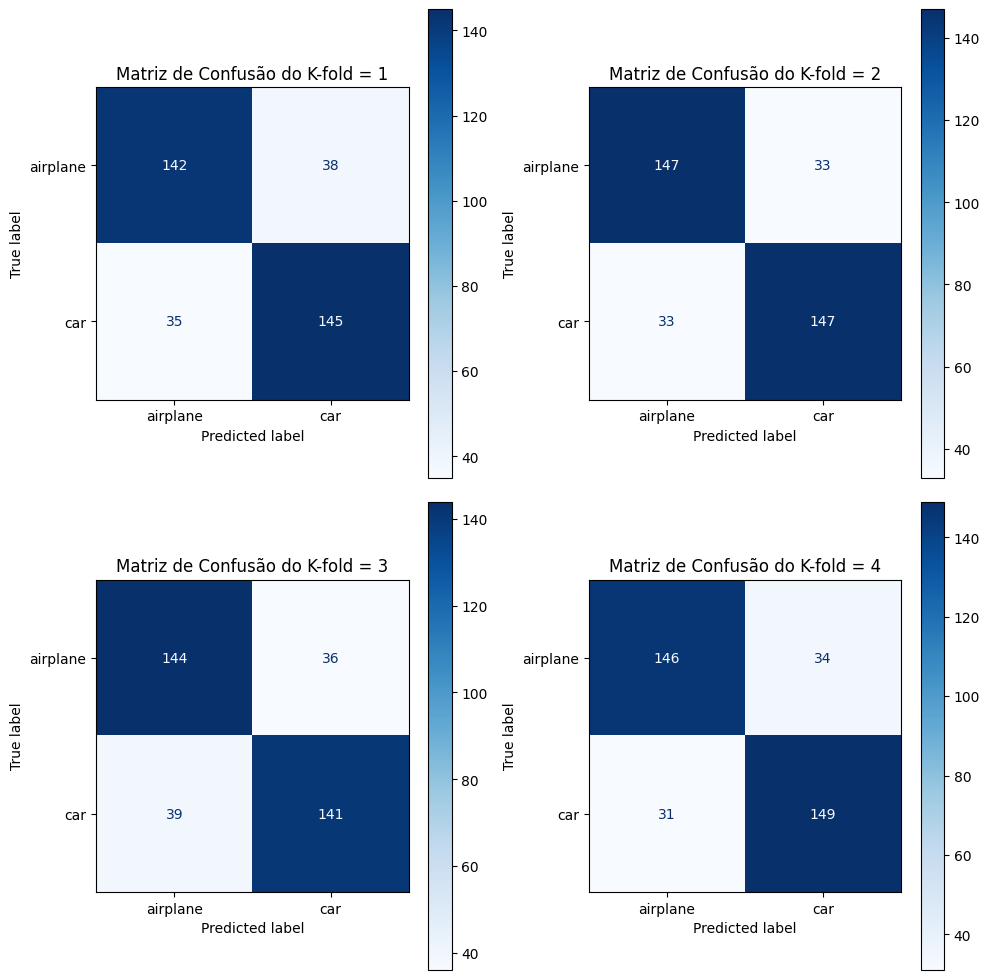
\includegraphics[width=0.95\textwidth]{imgs/ex3/conf3.png}
    \caption{Matriz de confusão dos modelos do item (a) aplicados ao conjunto de testes}
    \label{fig:conf3} % cria um rótulo para referência no texto
\end{figure}

\begin{figure}[H]
    \centering 
    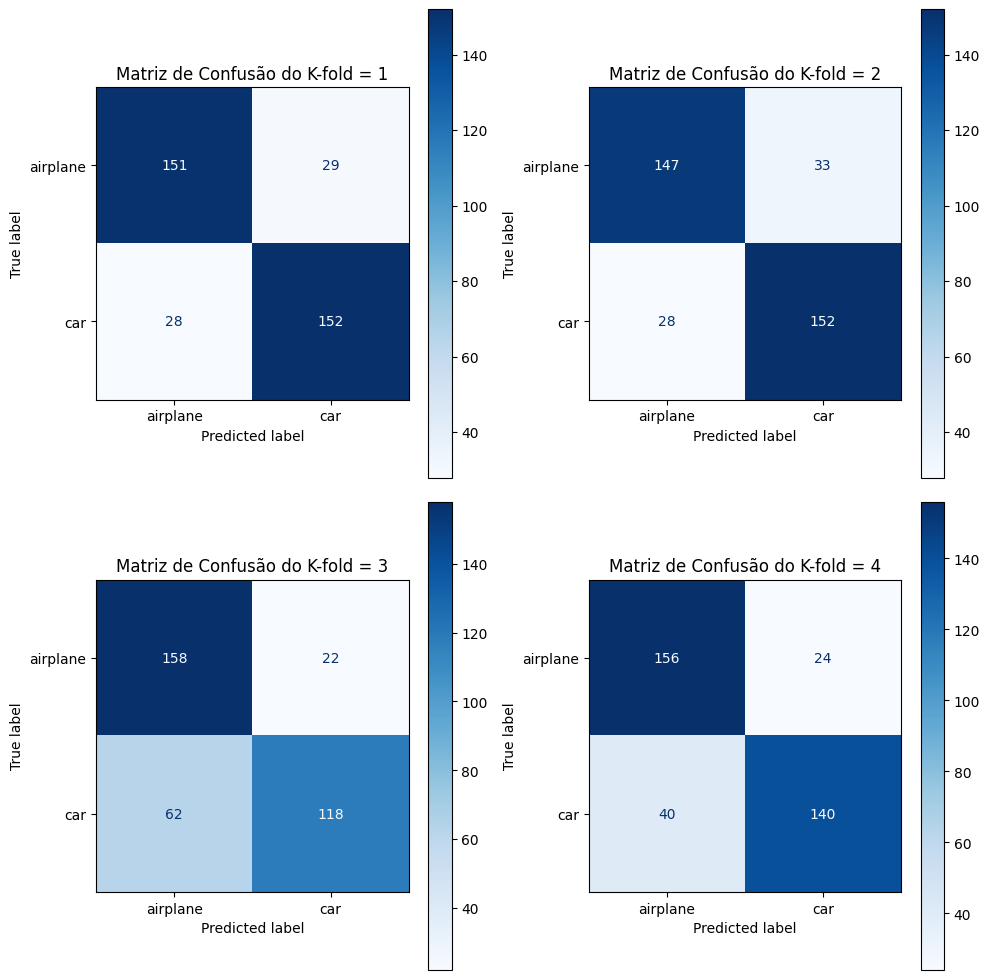
\includegraphics[width=0.95\textwidth]{imgs/ex3/conf4.png}
    \caption{Matriz de confusão dos modelos do item (b) aplicados ao conjunto de testes}
    \label{fig:conf4} % cria um rótulo para referência no texto
\end{figure}

Para acessar o código referente à realização deste exercício, \href{https://github.com/lorran-araujo/LNCC/blob/main/disciplinas/redes-neurais/codes/lista3/exercicio3.ipynb}{clique aqui}.

% ----------------------------------------------------------
% Referências bibliográficas
% ----------------------------------------------------------
\bibliography{Bibliografia}

\end{document}
